\documentclass[a4paper,ngerman]{scrartcl}

\usepackage{amsmath}
\usepackage{amsfonts}
\usepackage{amssymb}
\usepackage[utf8]{inputenc}
\usepackage{graphicx}
\usepackage[ngerman]{babel}
\usepackage{hyperref}
\usepackage{float}
\usepackage{caption}
\usepackage{subcaption}
\usepackage{multirow}  %for tables
\usepackage{icomma} % Handle german comma as decimal point in numbers
\usepackage{units,siunitx} % Write units with correct spacing
\usepackage{upgreek} % provide non-italic greek letters
\usepackage{url}
\usepackage{booktabs}
\usepackage{hepnames}
%\usepackage{subfig}

% Formatting of table & figure captions
\captionsetup{font={sf,footnotesize},labelfont=bf,textfont=sl,skip=6pt}
\setlength{\abovecaptionskip}{6pt}
\setlength{\belowcaptionskip}{0pt}

%locale for units to german
\sisetup{locale = DE}
\sisetup{separate-uncertainty=true}

\title{Landéfaktor}
\subtitle{Versuch vom 15. Dezember 2014}
\date{Letzte Änderung: \today}
\author{Michel Rausch, Michael Eliachevitch}

\begin{document}

\maketitle
\tableofcontents
\newpage

\section{Vorbereitung}

\subsection{Einleitung}
\label{sec:einfuhrung}
% Ziel: Bestimmung der Lebensdauer und des Landé-Faktors von Myonen, 
% Myonen sinde Sekundärteilchen der kosmischen Strahlung
% wir werden ständig mit Myonen bombardiert, ohne es zu merken


\subsection{Theoretische Grundlagen}
\label{sec:theorie}

\subsubsection{Enstehung von Myonen in Luftschauern}
\label{sec:luftschauer}

Die Erde wird ständig hochenergetischer kosmischer Strahlung getroffen. 
Diese besteht zu einem Großteil von 85\% aus Protonen, aber auch aus 12\% $alpha$-Teilchen und etwa 2\% schweren Kernen,
sowie einer elektromagnetischen Komponente mit Elektronen und Gammaquanten~\ref{ref:bb}.
Aus Experimenten ist bekannt, dass die kosmische Strahlung ein Potenzspektrum der Form

\begin{equation}
  N(> E) = K \cdot \left(\frac{E}{E_0}\right)^{-\gamma}
  \label{eq:powerlaw}
\end{equation}
hat, mit $E_0 = \SI{e16}{eV}$, $K = \SI{3e4}{\per\square\meter\per\hour}$ und dem Exponenten $\gamma$ in einem Bereich zwischen 1,7 und 2,1.
Wenn man das Spektrum doppelt logarithmisch aufträgt, erhält man eine Gerade mit einer dem Faktor $\gamma$ entsprechenden Steigung.
Bei $\SI{4e15}{eV}$ wird $gamma$ etwas größer, was als "`Knie"' bezeichnet wird, und etwa $\SI{e18}{eV}$ wird der Faktor $gamma$ wieder etwas kleiner, was als "`Knöchel"' bezeichnet wird. Eine Hypothese ist, dass diese Struktur mit dem Übergang von galaktischer zu extragalaktischer kosmischer Strahlung zusammenhängt. In Abbildung~\ref{fig:cr_spectrum} ist das Spektrum des kosmischen Strahlung mit den neuesten Messwerten von den aktuellen Luftschauerexperimenten dargestellt. Zu beachten ist, dass es sehr steil ist, weshalb es mit einem Faktor $E^{2,6}$ multipliziert wird. Die Folge für die Beobachtung von kosmischen Strahlen ist, dass der Fluss bei hohen Energien sehr selten wird. Daher bietet es sich bei der
Beobachtung an, die Atmosphäre als Detektor mit einer sehr hohen effektiven Fläche zu verwenden und die kosmischen Teilchen ähnlich wie bei einem Kalorimeter anhand der Luftschauer zu beobachten, die entstehen, sobald sie auf die Atmosphäre treffen.
 
\begin{figure}[tbh!]
  \centering
  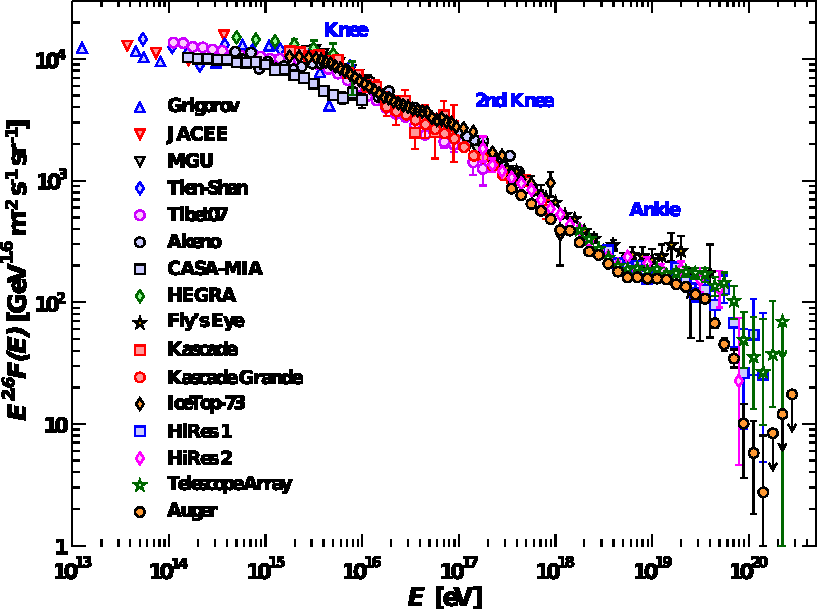
\includegraphics[width=0.8\textwidth]{abbildungen/cr_spectrum_pdg14.pdf}
  \caption{\textbf{Spektrum der kosmischen Strahlung für alle Teilchen aus den Daten von verschiedenen Luftschauerexperimenten.} Aufgetragen ist der differentielle Fluss, gewichtet mit der Energie $E^{2,6}$, gegen die Teilchenenergie pro Nukleon. Gut zu sehen sind das Knie bei etwa $\SI{4e15}{eV}$ und der Knöchel ab $\SI{e18}{eV}$, was die beiden Punkte sind, bei denen sich der Faktor $\gamma$ des Potenzspektrums der kosmischen Strahlung ändert. Mit den neusten experimentellen Daten scheint es auch einen zweites Knie bei $\SI{e17}{eV}$ zu geben. Stand 2014 \ref{ref:pdg14}.}
  \label{fig:cr_spectrum}
\end{figure}

Trifft ein hadronisches Teilchen auf die Atmosphäre, erzeugt es einen hadronischen Luftschauer, bei dem durch hadronische Wechselwirkungen
zu einem Großteil Pionen, aber auch Kaonen entstehen, die durch weitere Zusammenstöße mit Kernen noch mehr Pionen und Kaonen entstehen lassen,
sodass man eine Kaskade von Teilchen erhält. 
Neutrale Pionen zerfallen sehr schnell in zwei Gammaquanten, die durch Paarbildung und Bremmstrahlung elektromagnetische Subschauer entstehen lassen

\begin{equation}
\Pgpz \rightarrow \Pgamma + \Pgamma.
\end{equation}

Geladene Pionen, die ein Drittel der entstehenden Pionen betragen, zerfallen größtenteils in Myonen und Myon-Neutrinos:
\begin{equation}
  \begin{split}
    \Pgpp &\rightarrow \APmuon + \Pgngm  \\
    \Pgpm &\rightarrow \Pmuon + \Pagngm \\
  \end{split}
\label{eq:pipmdecay}
\end{equation}

Der Zerfallskanal in Elektronen und Elektron-Neutrinos ist stark unterdrückt, auch wenn er energetisch günstiger wäre. 
Das liegt daran, dass die schwache Wechselwirkung, der dieser Zerfall unterliegt, eine vektorielle Kraft ist, genauer gesagt
eine sogenannten V-A-Wechselwirkung (\emph{Vektor-Axialvektor-Wechselwirkung}).
Sie koppelt nur an linkshändige Teilchen und rechtshändige Antiteilchen, womit sie stark paritätsverletztend ist.
Damit sind Neutrinos immer linkshändig und Antineutrinos immer rechtshändig, da sie nur schwach wechselwirken und nahezu masselos sind.
Aus der Impulserhaltung folgt, dass das in~\ref{eq:pipmdecay} im Zerfall entstehende Myon bzw. 
Elektron in die entgegengesetzte Richtung wie
das Neutrino emittiert werden muss. 
Da der Drehimpuls auch erhalten ist, muss zum Beispiel bei einem emittierten rechtshändigen Antineutrino das Elektron bzw. 
Myon ebenfalls rechtshändig sein. 
Da Elektronen eine sehr geringe Masse $m_e = \SI{511}{keV}$ haben, bewegen sie sich bereits bei niedrigen Impulsen fast mit Lichtgeschwindigkeit und treten daher meist linkshändig auf. 
Die rechtshändige Komponente ist dagegen stark unterdrückt. 
Myonen haben eine ungefähr 200-fach höhere Masse als Elektronen, weshalb die Wahrscheinlichkeit bei ihnen viel höher ist, dass sie auch rechtshändig auftreten. 
Aufgrund des viel höheren Phasenraums für den Zerfall in Myonen, zerfallen geladene Pionen nur mit einer Wahrscheinlichkeit von $\SI{1,230+-0,004}{}$~[\ref{ref:pdg14}] in Elektronen.


Freie Myonen haben eine Lebensdauer von 
\begin{equation}
 \tau = \SI{2,197}{\micro\s}. [\ref{ref:pdg14}]
 \label{eq:lebensdauer}
\end{equation}

In dieser Zeit legen sie eine Strecke von $c_0 \cdot \tau \approx \SI{600}{m}$ zurück. 
Da sie normalerweise in mehreren Kilometern Höhe entstehen, würden sie mit einer solchen Lebensdauer im Laborsystem gar nicht bis
auf die Erdorberfläche treffen. Durch ihre hohe Energie haben sie im Laborsystem der Erde durch den Lorentz-Boost eine deutlich höhere Lebensdauer

\begin{equation}
  \tau_E = \gamma\cdot\tau,
\end{equation}
mit dem Lorentz-Faktor $\gamma = \frac{E}{E_0}$. Bei einer Energie von $E = \SI{10}{GeV}$ beträgt da Gamma-Faktor zum Beispiel
\begin{equation}
\gamma \approx \frac{\SI{10}{\giga\electronvolt}}{\SI{140}{\mega\electronvolt}} \approx 71, 
\end{equation}
was die Flugstrecke 71-Fach erhöhen würde, sodass sie normalerweise Problemlos die Erdoberfläche erreichen, wenn man annimmt, dass sie bis dahin nicht wechselwirken. Auf die Wechselwirkung von Myonen mit Materie wird jedoch im nächsten Kapitel eingegangen.


\subsubsection{Abbremsung von Myonen in Materie}
\label{sec:wwmitmaterie}
Ein weiterer Grund, warum so viele Myonen auf der Erde ankommen, ist, dass sie bei Energien unter GeV-Bereich, anders als Elektronen,
kaum Strahlungsverluste haben, da der Strahlungsverlust durch Bremmstrahlung, der sowas ist wie die Synchrotronstrahlung im Feld der Kerne,
ebenso wie die Synchrotronstrahlung, gemäß der Larmor-Formel proportional ist zu $m^{-4}$~\ref{ref:pdg14}. 
Bei mittleren Energien verlieren sie ihre Energie hauptsächlich durch Ionisation. 
Da Myonen somit in der Atmosphäre viel weiter kommen als Elektronen, macht dies möglich, durch die Messung des Verhältnisses der Anzahl von atmosphärischer Elektronen zu Myonen die Höhe des Schauermaximums abzuschätzen, da bei einem hohen Schauermaximum die meisten Elektronen auf dem Weg zur Erde absorbiert werden, während die Myonen eher den Erdboden erreichen.


Myonen werden oft als "`minimal ionizing particles"' (\emph{mips}) bezeichnet, da ihr Energieverlust durch Ionisation bei Energien im GeV-Bereich 
in der Nähe des Minimums der Bethe-Bloch Formel liegt. 
Bei Impulsen im MeV-Bereich~\ref{ref:pdg14} tritt jedoch der Bragg-Peak ein und sie verlieren 
auf kurzem Raum den Großteil ihrer Energie. 
Da sie bei niedrigen Energien nicht mehr dem Lorentz-Boost unterliegen, kann die Messung der Lebensdauer näherungsweise ab dem Zeitpunkt des Einfangs erfolgen. 
Dabei muss jedoch beachtet werden, ob man positive oder negative Myonen hat.
Positive Myonen können Elektronen aus den Kernhüllen einfangen und bilden so Myonium, eine wasserstoffähnliches Gebilde, wobei im Gegensatz zum Wasserstoff der Masserschwerpunkt genau zwischen den beiden Teilchen liegt und die effektiven Massen dabei sozusagen halbiert sind.
Die Lebensdauer des Myons bleibt bei diesem Prozess unverändert.
Negative Myonen hingegen können dagegen von den positiven Atomkernen in der K-Schale gefangen werden, da sie durch ihre unterschiedliche 
Teilchenart nicht durch das Pauli-Prinzip von den Elektronen blockiert werden. 
Von da können sie analog zum Elektroneinfang mit einem Proton schwach wechselwirken und dies damit in ein Neutron umwandeln. 
Aufgrund von diesem Prozess haben negative Myonen in Materie eine deutliche niedrigere Lebensdauer, in Kupfer zum Beispiel
\begin{equation}
\tau_{\Pmuon, \mathrm{Kupfer}} = \SI{0,163}{\micro\s}.\ [\ref{ref:bb}]
\label{eq:mumin-lebensdauer}
\end{equation}
Da man bei der Messung der Lebensdauer dadurch eine Überlagerung zweier Lebensdauern bekommt, ist es geschickt, bei der Messung nur die Ereignisse zu verwenden, bei denen das Signal aus dem Zerfall erst eine Sekunden nach dem Myonen-Trigger kommt, da dann die negativen Myonen größtenteils zerfallen sind.



\subsubsection{Polarisation von Myonen}
\label{sec:polarisation}

In~\ref{sec:luftschauer} wurde bereits erklärt die Paritätsverletzung der schwachen Wechselwirkung erklärt und warum Myonen nach der 
V-A-Theorie meist in Myonen und Myon-Neutrinos statt in Elektronen und Elektron-Neutrinos zerfallen.


Nun wollen wir betrachten, welchen Energie Myonen aus dem Zerfall erhalten und wie diese von der Zerfallsrichtung abhängt.
Aus der Energie- und Impulserhaltung folgt, dass das Myon im Ruhesystem des Pions eine Energie von 
\begin{equation}
  W_{\Pgm} = \frac{(m_{\Pgm} c^2)^2+(m_{\Pgp} c^2)^2}{m_{\Pgp} c^2}
\end{equation}
hat. 
Mit $m_{\Pgm} \approx \SI{106}{MeV}$ und $m_{\Pgp} \approx \SI{140}{MeV}$ erhält man damit eine Gesamtenergie von
$W_{\Pgm} \approx \SI{110}{MeV}$, womit das Myon zusätzlich zu seiner Ruheenergie eine kinetische Energie von $\SI{4}{MeV}$ erhält, das jedoch im Ruhesystem des Pions.
Im Laborsystem der Erde haben die Myonen unterschiedliche Energien, da sie in unterschiedliche Richtungen emittiert werden können.
In Richtung der Erde emittierte Myonen haben bei gleicher Pionenenergie eine höhere kinetische Energie als in entgegengesetzte Richtung emittierte Myonen. 
Da die Myonen in unterschiedliche Richtungen zerfallen können und auch die Einfallsrichtung der Pionen aus den Luftschauern einer Verteilung folgt,
erhält man folglich ein kontiunierliches Energiespektrum.


Da Myonen auf dem Weg zum Detektor auf der Erdoberfläche kontiunierlich Energie verlieren, muss ihre anfängliche Energie in einem beschränkten Bereich gelegen haben, da sie sonst nicht auf der Erde ankommen würden. 
Sie könnten von Pionen niedrigerer Energie stammen, bei denen die Myonen in Vorwärtsrichtung emittiert wurden oder von höherenergetischen Pionen, bei denen die Myonen in Rückwärtsrichtung emittiert wurden. 
Wenn das Spektrum der Pionen, welche zur kosmischen Sekundärstrahlung gehören, analog zur kosmischen Primärstrahlung, gemäß Gleichung~\eqref{eq:powerlaw} einem Potenzgesetz folgt, müsste es mehr niederenergetische Pionen geben, weshalb entsprechend der Anteil der in Vorwärtsrichtung emittierten Myonen größer müsste, als der Anteil der Rückwärtsrichtung emittierten Myonen.


Um zwischen den in Vorwärts- und in Rückwärtsrichtung emittierten Myonen unterscheiden zu können, muss deren Polarisation betrachtet werden.
Negative Myonen aus dem Pionenzerfall sind rechtshändig und damit bei Emission in Vorwärtsrichtung auch in Vorwärtsrichtung polarisiert. 
Die positiven Myonen $\APmuon$ sind dagegen rechtshändig und daher würde man bei ihnen bei Emission in Vorwärtsrichtung eine Polarisation in Rückwärtsrichtung erwarten. 
Da die negativen $\Pmuon$ gemäß \eqref{eq:mumin-lebensdauer} eine geringere Lebensdauer haben, werden wir hauptsächlich die positiven Myonen $\APmuon$ messen, und da diese mehrheitlich in Vorwärtsrichtung emittiert werden sollten, erwarten wir im Mittel eine Polarisation in Rückwärtsrichtung. 


Da die Abbremsung des Myons in ganz kurzer Zeit erfolgt (Bragg-Peak), erfolgt die Depolarisation im thermalisiertem Zustand, da es darin die meiste Zeit bis zum Zerfall verbringt. 
Die genauen Prozesse hängen von dem Material statt, in dem die Absorption stattfindet.
Im Kupfer erfolgt die Depolarisation wie in anderen paramagnetischen Metallen durch inhomogene Magnetfelder der Kernmomente und durch magnetische Verunreinigungen~\ref{ref:bb}, wobei die Relaxationszeit in diesen Metallen lang ist gegenüber der Myonenlebensdauer und etwa $\SI{50}{\micro\s}$ beträgt~\ref{ref:bb}.


\subsubsection{Nachweis des Myonenzerfalls}
\label{sec:nachweis}
% die theorie hiervon kann ich auch noch nicht gut (michael)
% aber müsste nicht viel sein


Durch das emittierte Positron wird der Zerfall gekennzeichnet. Das Spektrum kann differentiell im Raumwinkel $\Omega$ beschrieben werden in der Form

\begin{equation}
\label{eqn:doppeldiffspektrum}
\frac{d^2N}{d\epsilon d\Omega} = \frac{\epsilon^2}{2 \pi} \cdot \left[  (3- 2\epsilon) - P \cdot (1-2\epsilon) \cdot \cos(\theta)  \right] = \frac{3 \epsilon^2 - 2 \epsilon^3}{2 \pi} \cdot \left[  1 + P \cdot \frac{2 \epsilon -1}{3 - 2\epsilon} \cdot cos(\theta)  \right] .
\end{equation}

Hierbei ist $P$ die Polarisation, $\theta$ der Winkel zwischen Impuls und Spin des Myons. $\epsilon = E / E_{max}$ ist eine Energie in Einheiten der maximalen Energie $E_{max} = m_{\mu}c^2/2$, die beim Zerfall auf das Myon übertragen werden kann. 

Obige Gleichung lässt sich vereinfacht schreiben als

\begin{equation}
\frac{d^2N}{d\epsilon d\Omega} = a \cdot (1 + b \cdot cos(\theta) ) .
\end{equation}

$b$ läuft von $-\frac{1}{3}$ über $0$ bis $1$. Die Emission des Positrons ist demnach nicht isotrop bezüglich des Spins des $\mu^{+}$. Sie erfolgt bevorzugt in dessen Richtung. Bei höheren Energien ist die Asymmetrie größer. Es existiert eine untere Schwelle für Beobachtung der Positronen. Solche mit zu geringer Energie erreichen den Detektor nicht. 

Wird Gleichung \ref{eqn:doppeldiffspektrum} über $\epsilon$ integriert, erhält man

\begin{equation}
\label{eqn:spektrum}
\frac{dN}{ d\Omega} = k \cdot (1 + A \cdot cos(\theta) ).
\end{equation}

$k$ ist eine Konstante, die durch die Schwelle bestimmt wird. $A$ wird als Asymmetrie bezeichnet. Wird über das ganze Spektrum integriert, so ist $A=P/3$, für die obere Hälfte erhält man $A = 0.44 \ P$, der Grenzwert beträgt für hohe Schwellen $A=P$. Bei höheren Schwellen sinkt die Zählrate jedoch ab, sodass zwischen hoher Asymmetrie und Zählrate abgewägt werden muss.

Gleichung \ref{eqn:spektrum} wird über einen endlichen Winkel integriert, um die Winkelverteilung der Positronen zu berücksichtigen. Die Asymmetrie nimmt durch die Mittelung über $\theta$ ab.







\subsubsection{Präzession von Myonen im Magnetfeld}
\label{sec:prazission}
% gyromagnetische verhältnis gamma, landé-faktor g erklären
% präzission im magnetfeld
% am wichtigsten ist eigentlich nur folgende gleichung:
%\begin{equation}
%g = \frac{\gamma \hbar}{\mu_\mathrm{B}} = \frac{\hbar \omega}{\mu_\mathrm{B}\mathrm{B}}
%\end{equation}

Das Magnetische Moment $\vec{\mu}$ steht mit dem Drehimpuls $\vec{J}$ eines Teilchen in Relation

\begin{equation}
\vec{\mu} = \gamma \cdot \vec{J} .
\end{equation}

Aus der Bewegungsgleichung im Magnetfeld $\vec{B}$

\begin{equation}
\frac{d\vec{J}}{dt} = \vec{\mu} \times \vec{B}
\end{equation}

folgt die Präzessionsfrequenz

\begin{equation}
\omega = \gamma \cdot B
\end{equation}

mit dem Betrag des Magnetfeldes $B$ und dem gyromagnetischem Verhältnis 

\begin{equation}
\label{eqn:praez_gyro}
\gamma = \frac{g \mu_B}{\hbar}. 
\end{equation}

Das Bohrsche Magneton $\mu_B$ ist für ein Teilchen der Masse m und der Ladung q

\begin{equation}
\mu_B = \frac{q\hbar}{2 m} .
\end{equation}


Für ein Elektron ergibt dies [\ref{ref:bb}]

\begin{equation}
\mu_B (Elektron) = \SI{9.273e-24}{ J/T } .
\end{equation}

Für das schwerere Myon beträgt es [\ref{ref:bb}]

\begin{equation}
\mu_B (Elektron) = \SI{4.485e-26}{ J/T } .
\end{equation} 


Der dimensionslose Faktor $g$ wird als \textbf{Landé-faktor} bezwichnet. Für den Bahndrehimpuls ist er genau gleich eins. Für den Spin ist er 2 + Korrekturen höherer Ordnung. Nach Gleichung \ref{eqn:praez_gyro} lässt er sich berechnen mit

\begin{equation}
g = \frac{\gamma \hbar}{\mu_B} = \frac{\hbar \omega}{\mu_B B} .
\end{equation}


\subsubsection{Messprinzip}
\label{sec:messprinzip}
% zerfall von myonen erfolgt exponentialgesetz
% wie misst man präzission?
% -> angelegtes magnetfeld
% formeln...

\subsubsection*{Messung der mittleren Lebensdauer}

Die Messung startet mit der Registrierung der Abbremsung eines Myons im Detektor. Durch den Zerfall entsteht ein Positron, dessen Auftreten die Messung stoppt. Da es sich um einen Zerfall handelt, kann man für viele beobachtete Myonen ein Exponentialgesetz ansetzen:

\begin{equation}
\label{eqn:messprinzip-zerfall}
N(T) = N_0 \cdot \exp(-t / \tau) .
\end{equation} 
	
$N_0$ ist die Gesamtzahl der im Detektor registrierten, gestoppten Myonen während der Messzeit, $N$ die Anzahl der beobachteten Zerfälle.
Die mittlere Lebensdauer $\tau$ kann man bestimmen, auch ohne die Energie und Richtung der Myonen zu betrachten. 

\subsubsection*{Messung der Präzessionsfrequenz}


Über das Stopptarget wird ein Magnetfeld transversal zur Einfallsrichtung der Myonen gelegt, in dem diese präzedieren.
Indem nur in eine bestimmte Richtung emittierte Positronen gemessen werden, ist die Zählrate mit der Präzessionsfrequenz moduliert. Ist der Spin der Myonen antiparallel zur Richtung, ist er am geringsten, bei parallel gerichtetem am höchsten.


Gleichungen \ref{eqn:spektrum} und \ref{eqn:messprinzip-zerfall}
lassen sich zusammenfassen zu

\begin{equation}
N(t) = K \cdot \exp(- \frac{t}{\tau}) \cdot \left[ 1 + \overline{A} \cdot \cos(\omega t + \delta) \right] .
\end{equation}

Die Exponentialfunktion entstammt dem Zerfallsgesetz aus Gleichung \ref{eqn:messprinzip-zerfall}, der Term in der eckigen Klammer beschreibt die Modulation durch Präzession.
$\overline{A}$ ist die über die Geometrie des Detektors gemittelte Asymmetrie. Diese ist aufgrund der Depolarisation der $\mu^{+}$ zeitabhängig und folgt einem Exponentialgesetz

\begin{equation}
\overline{A} = \overline{A}_0 \cdot \exp(- \frac{t}{ T_R }) .
\end{equation}

In Kupfer kann sie jedoch als konstant angenommen werden. $T_R$ bezeichnet die Relaxationszeit.
	
\clearpage

\subsection{Versuchsaufbau und Durchführung}
% von oben nach unten: Szinti 1, Szinti 2, Kupferabsorber in Magnetfeld, Szinti 3
% Koinzindenz und Veto-Schaltung erklären: 
% D.h. Wir nehmen nur die Ereignisse, wo 1 und 2 gleichzeitig ausschlagen (Koinzindenz) und 3 NICHT ausschlägt (Veto bzw Antikoinzindenz)
% erklären was ein diskriminator in der analog-digitalwandlung ist und wie die schwelle (trigger) eingestellt werden muss:
% trigger muss so sein, dass untergrund unterdrückt wird und man nur hauptsignal sieht
% zu hoher trigger verringer unnötig statistik
% trigger für veto (szinti 3) lieber etwas niedriger als zu hoch, damit man keine falschen ereignisse aufnimmt
% was ist ein TAC (zeit-amplituden-converter) und zeiteichung ?

In Abbildung \ref{fig:aufbau_skizze} ist eine Skizze des Versuchsaufbaus gezeigt. Drei Szintillatorplatten, mit einer Dicke von $\SI{2.5}{\centi\meter}$, sind waagerecht übereinandergelegt. Zwischen dem zweiten und dritten befindet sich eine ebenso dicke Kupferplatte, welches die Myonen stoppt. 
Signale aus den Szintillatoren werden mit einem Photomultiplier (PM) verstärkt und in die Koinzidenzschaltung geschickt.
Ein gestopptes Myon hat die Signatur $1 + 2 + \overline{3}$, also eine Koinzidenz der oberen Szintillatoren und eine Antikoinzidenz des unteren. Damit wird die Messsung begonnen. Die Messung wird beendet, wenn ein Positron detektiert wird. Dieses kann in Richtung des Szintillators 2, oder 3 emittiert werden. Das Stoppsignal auszusenden, wenn eines der beiden Szintillatoren ein Signal aussendet ist jedoch nicht optimal, da zufällige Stopps aufgrund von Hintergrundstrahlung auftreten. Am besten eignet sich eine Signatur $1 + 2 + \overline{3}$. Die Zählrate ist hier jedoch abgeschwächt.  


\begin{figure}[tb!]
  \centering
  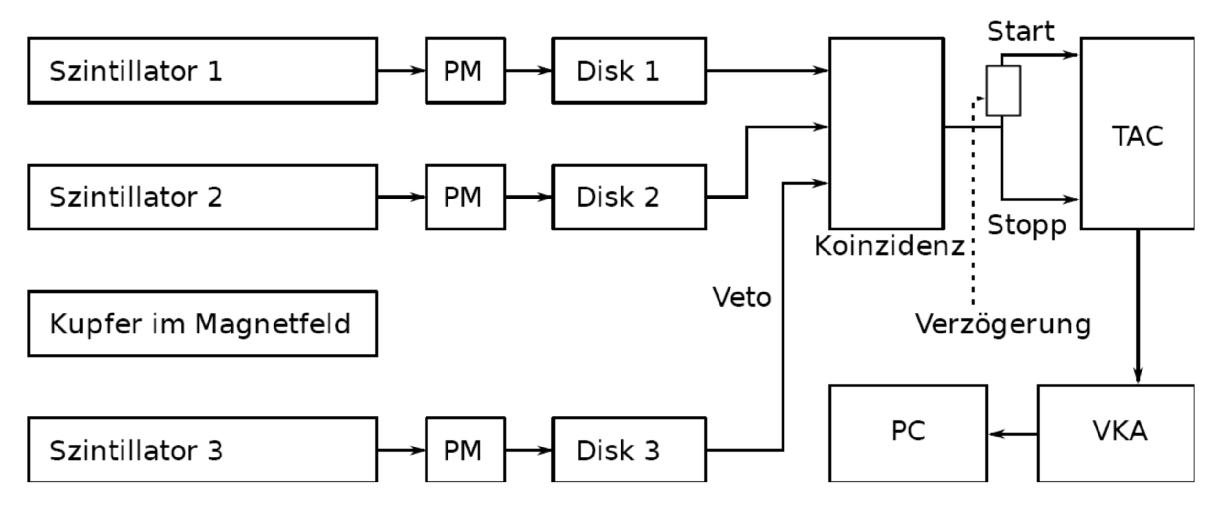
\includegraphics[width=1\textwidth]{abbildungen/aufbau_skizze.png}
  \caption{\textbf{Skizze des Versuchsaufbaus.} 
  \\ 
  Drei Kunstoffszintillatoren und eine Kupferplatte mit einer Dicke von jeweils $\SI{2.5}{cm}$ sind übereinander angeordnet. Die Kupferplatte befindet sich zwischen dem 2. und 3. Szintillator. Das Signal aus den Szintillatoren wird mit Photomultpliern (\textbf{PM}) verstärkt. Bei den definierten Signatur wird von der Koinzidenz ein Signal für den Start, bzw. Stopp der Messung gegeben. Das Startsignal wird um einige Nanosekunden verzögert, damit der Time to Amplitude Converter (\textbf{TAC}) das Signal verarbeiten kann. Über einen Vielkanalanalysator (\textbf{VKA}) wird das Signal an einem Rechner (\textbf{PC}) analysiert.
  \\Quelle: [\ref{ref:bb}]}
  \label{fig:aufbau_skizze}
\end{figure}

Der Time to Amplitude Converter (TAC) kann Signale nicht verarbeiten, wenn diese gleichzeitig eintreffen. Da Start- und Stoppsignal die selbe Signatur haben, ist dies der Fall. 
Daher wird das Startsignal um einige Nanosekunden verzögert. 
Das verzögerte Startsignal eines Myons startet den Zähler, wird aber nicht von dessen Stoppsignal gestoppt. Das nächste Stoppsignal kommt erst bei dem nächsten Myon. Hier liegt das Stoppsignal aufgrund der Verzögerung schneller an, als dessen Startsignal. Seit $T_{12}$ die Zeit, die zwischen dem Eintreffen der beiden Myonen vergangen ist, $\tau_1$ und $\tau_2$ die Lebensdauern der beiden Myonen und $\delta t$ die Verzögerung am Startsignal. 

Ohne Verzögerung und mit einem entsprechend schnellen Detektor würde ein Startsignal kommen, gefolgt von dem Stoppsignal für jedes Myon. Man würde die Lebensdauer also direkt messen, was aber hier nicht möglich ist. Stattdessen misst man die Zeit von dem verzögertem Startsignal des ersten bis zu dem Stoppsignal des zweiten Myons. Die gemessene Zeit ist also

\begin{equation}
t = T_{12} - \tau_2 .
\end{equation}

Das Startsignal des zweiten Myons wird ignoriert, denn der TAC benötigt einige Microsekunden, um das analoge Signal zu erzeugen.



\subsubsection{Zusätzliche Aufgaben}

\begin{itemize}
\item a) Einstellung der Schwellen an den Diskriminatoren
\item b) Zeiteichung des Zeit-zu-Amplituden-Konverters (TAC)
\end{itemize}

\newpage

\section{Auswertung}

\subsection{Zeitkalibrierung}

Ein Funktionsgenerator wurde an den Starteingang des TAC geschlossen, sowie über Verzögerungsglieder an den Stoppeingang. Diese wurden zugeschaltet, um die Zeitverzögerung in bekannten Schritten von \SI{1}{\micro\second} zu erhöhen. Die Breite der zugehörigen Peaks war klein gegenüber deren Abstand, sodass die Messungen sich in einer einzelnen Grafik, Abb. \ref{fig:zeitkalibrierung_hist}, auswerten ließen. Die Nummer des Kanals steigt mit der zugehörigen Verzögerung. 

\begin{figure}[tb!]
\centering
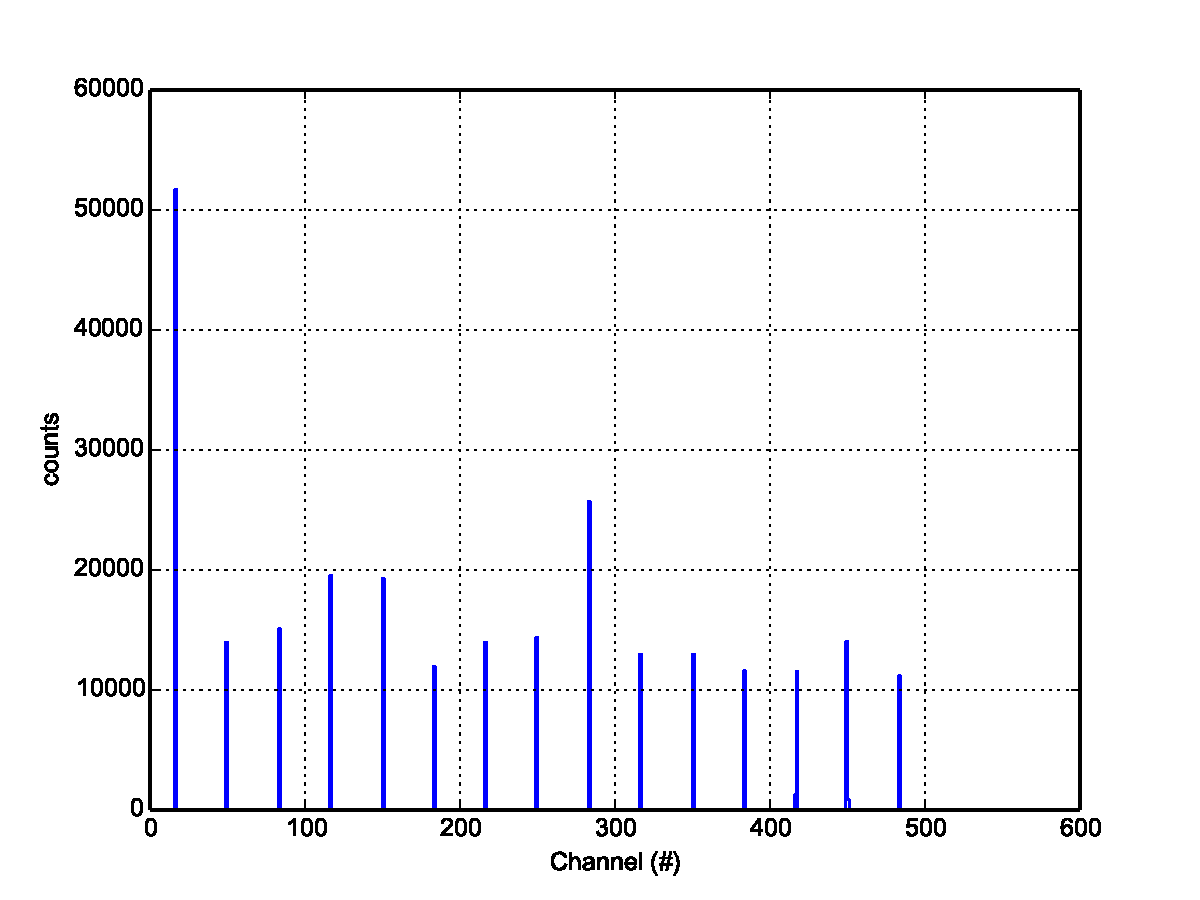
\includegraphics[width=0.7\textwidth]{abbildungen/zeitkalibrierung_hist.pdf}
\caption[Daten zur Zeitkalibrierung]{\textbf{Daten zur Zeitkalibrierung.} Die gezeigten Peaks gehören zu Signalen, die durch Einstellen von unterschiedlichen Verzögerungszeiten am Funktionsgenerator entstanden sind.
Die Breite der Peaks war groß gegenüber dem Abstand und lag im Bereich einer Kanalbreite, sodass sich die Messungen in einer einzelnen Grafik auswerten ließen.
Die Kanäle entsprechen der Zeit, die nach rechts hin zunimmt.
Die Peaks sind äquidistant und sollten durch die eingestellten Zeitverzögerungen einen Abstand von \SI{1}{\micro\second} haben, sodass sich damit eine Zeitkalibrierung der Kanäle durchführen lässt.}
\label{fig:zeitkalibrierung_hist}
\end{figure}


Mittels des Python-Moduls \emph{numpy} wurde ein linearer Fit durchgeführt. Aus der der daraus resultierenden Geradensteigung erhält man eine Zuordnung von Zeit zu Kanal. Die Regression ist in Abbildung \ref{fig:zeitkalibrierung} gezeigt, das Ergebnis lautet

\begin{equation}
\label{eqn:Zeitkalibrierung}
\mathrm{Zeit(\#Kanal)} = \mathrm{\#Kanal} \cdot \SI{29.9783924  +-  0.0000004 }{\nano\second}
+ \SI{489.41+-0.04}{\nano\second}~.
\end{equation}

Der Fehler der in der Steigung der Zeitkalibrierung ist im Vergleich zu den anderen
Fehlern vernachlässigbar klein und wird im folgenden daher nicht
weiter fortgepflanzt, während der Fehler im y-Achsenabschnitt von \SI{0.04}{\nano\second}
beibehalten wird.

\begin{figure}[tb!]
\centering
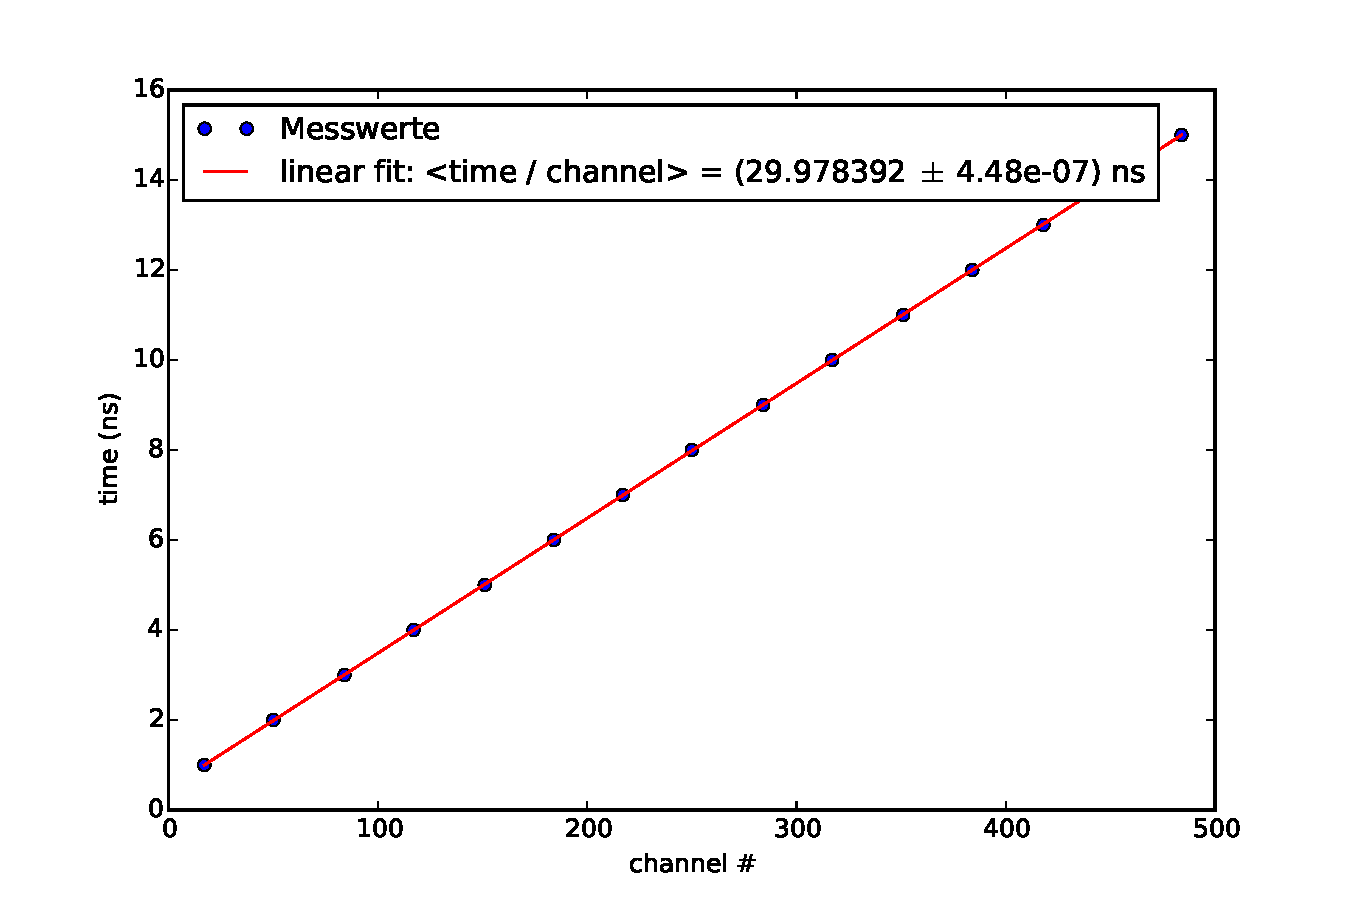
\includegraphics[width=0.7\textwidth]{abbildungen/zeitkalibrierung.pdf}
\caption[Zeitkalibrierung]{\textbf{Zeitkalibrierung.} Mittels eines Pythonscripts wurde ein linearer Fit durchgeführt. Die Kanalnummer des VKAs wurde auf der x-Achse aufgetragen, die dazugehörige Verzögerung auf der y-Achse. Mit der Geradengleichung wurden Kanäle einer Zeit zugeordnet.}
\label{fig:zeitkalibrierung}
\end{figure}



\subsection{Magnetfeld}

Zur Bestimmung des Magnetfeldes im Inneren in der Spule wurde eine Hallsonde verwendet.
Die darin entstehende Hallspannung wurde einem Vorwiderstand gemessen,
weshalb wir sie $U_{\mathrm{VW}}$ nennen.
Die Kalibrierung von gemessener Spannung zu magnetischem Fluss $B$ war bereits vorher durchgeführt worden,
weshalb das Magnetfeld über folgende Formel berechnet werden kann:
\begin{equation}
\label{eqn:B-gauss}
B \mathrm{/G} = -1,68946 + 0,30472 \cdot U_{\mathrm{VW}} \mathrm{/mV}~.
\end{equation}


In der Spule ist das Magnetfeld inhomogen. Der Fehler für die Inhomogenität wurden aus der übernommenen Messreihe in Tabelle \ref{tab:fieldinhomogenities} ermittelt. Es sind die Spannungen an der Hallsonde aufgelistet. Diese stehen in einem linearen Verhältnis zu der Magnetfeldstärke, daher können die relativen Fehler übernommen werden. 
Der relative Fehler wurde über die Standwardabweichung aller Messwerte, geteilt durch deren Mittelwert, bestimmt, wobei die Randbereiche aus der Messung rausgenommen wurden. Damit erhielten wir

\begin{equation}
\label{eqn:inhomogen_fehler}
\sigma_{\rm B} = 0,067 \approx 7\% ~.
\end{equation}

Die Spannung am Vorwiderstand betrug, mit einem relativen Fehler von $\sigma_{\rm VW} = 3\%$
%(* 123.6 0.03)3.7079999999999997
\begin{equation}
U_{\mathrm{VW}} = \SI{123,6+-3.7}{\milli \volt} \approx \SI{123+-4}{\milli \volt} ~.
\end{equation}

Hieraus ergab Formel \eqref{eqn:B-gauss}, mit dem Fehler der Inhomogenität aus Gleichung \eqref{eqn:inhomogen_fehler}
und dem Fehler der Spannung im Vorwiderstand $\sigma_{\rm VW} = 3\%$
\begin{equation}
\label{eq:B}
B = \SI{36+-3}{G} ~.
\end{equation}
%(- (* 0.30472 123.6) 1.68946)
%(* 36.0 0.067)2.412
%(* 36.0 0.03)

\begin{table}[tb!]
\centering
\caption[Inhomogenität des Magnetfelds der Spule]{\textbf{Inhomogenität des Magnetfelds der Spule.} 
Um den relativen Fehler des Magnetfeldes im inneren der Spule zu bestimmen, wurde auf vorliegende Messungen einer Hallsonde zurückgegriffen.
Bei verschiedenen Stellen entlang der Längsachse der Spule bei einem Abstand von $l$ zum Anfang der der Spule 
wurde die Spannung an der Hallsonde gemessen.
Für jeden dieser Punkte wurden vier Messwerte für verschiedene radiale Abstände von der Längsachse der Spule aufgenommen.
Die mit "'*"' markierten Werte für $l = \SI{0.00}{m}$ und $l = \SI{1.00}{m}$ wichen stark von den anderen Werten ab,
wurden daher nicht in die Berechnung des Fehlers aufgenommen.}
\begin{tabular}{ccccc}
\toprule 
$l$/m	&	$U_{\mathrm{Hall}} (0 \mathrm{m})$/mV	&	$U_{\mathrm{Hall}} (0,28 \mathrm{m})$/mV	&	$U_{\mathrm{Hall}}(- 0,28 \mathrm{m})$/mV	&	$U_{\mathrm{Hall}} (0 \mathrm{m})$/mV	\\
\midrule
0,00* & 149,6* & 123,6* & 123,6* & 139,7* \\
0,05 & 213,9 & 231,2 & 227,5 & 218,8 \\
0,10 & 243,6 & 257,1 & 257,2 & 243,6 \\
0,15 & 247,3 & 267,0 & 267,0 & 248,5 \\
0,20 & 253,4 & 271,0 & 272,0 & 249,7 \\
0,25 & 272,0 & 279,4 & 279,4 & 262,1 \\
0,30 & 288,1 & 284,3 & 285,6 & 291,8 \\
0,35 & 283,1 & 283,1 & 284,3 & 284,3 \\
0,40 & 270,7 & 279,4 & 281,9 & 270,7 \\
0,45 & 269,5 & 279,4 & 280,6 & 269,5 \\
0,50 & 279,4 & 280,6 & 283,1 & 278,2 \\
0,55 & 289,3 & 283,1 & 285,6 & 290,5 \\
0,60 & 289,3 & 284,3 & 285,6 & 289,3 \\
0,65 & 264,6 & 278,2 & 278,2 & 260,9 \\
0,70 & 273,2 & 279,4 & 280,6 & 273,2 \\
0,75 & 270,7 & 280,6 & 280,6 & 274,5 \\
0,80 & 259,6 & 274,5 & 274,5 & 257,2 \\
0,85 & 255,9 & 272,0 & 270,7 & 257,2 \\
0,90 & 243,6 & 262,1 & 260,9 & 244,8 \\
0,95 & 217,6 & 238,6 & 237,4 & 222,5 \\
1,00* & 157,0* & 160,7* & 155,8* & 163,2* \\
\bottomrule
\end{tabular}
\label{tab:fieldinhomogenities}
\end{table}


\clearpage
\subsection{Bestimmung der Lebensdauer des Myons}

Gemäß dem in der Vorbereitung in Abschnitt~3 besprochenen und in
Abbildung~2 gezeigtem Versuchsaufbau wurde die Lebensdauer der Myonen
gemessen. Gemessen wurde die Zeit zwischen dem Triggersignal im
Szintillator~1 (siehe Abb.~\ref{fig:aufbau_skizze}) und dem Signal aus dem Myonzerfall, welches durch dabei
emittierte Positron ausgelöst wurde. Es wurden nur solche Ereignisse
selektiert, bei denen das Positron nach oben emittiert wurde, sodass
wir mit dem angelegten Magnetfeld eine Modulation erhalten, die der
Präzession des Myons im Magnetfeld entspricht.

Um eine für die Auswertung ausreichende Statistik zu erreichen, ist
bei der in unserem Aufbau verwendeten sensitiven Detektionsfläche von ungefähr
\SI{1}{\square\meter} und dem kleinen Phasenraum der Messung eine
lange Messzeit von mehreren Tagen oder Wochen notwendig, um eine
ausreichende Statistik zu erhalten. Daher haben wir bereits vorhandene
Messwerte verwendet.

Die waren bereits als Histogramm gegeben, 
das heißt es war für jeden Kanal die Anzahl der Zerfälle in diesem Zeitintervall angegeben.
Dies  wurde mit dem Analyse-Framework ROOT geplottet, wie in
Abbildung~\ref{fig:zerfallszeiten} zu sehen ist. Das Histogramm  wurde dann mit
Gleichung~21 aus der Vorbereitung gefittet. Zur Erinnerung ist sie
hier noch einmal aufgeführt.

\begin{equation}
\label{eq:fitfkt}
N(t) = K \cdot \mathrm{e}^{- \frac{t}{\tau}} \cdot \left[ 1 + \overline{A} \cdot \cos(\omega t + \delta) \right] + const.~.
\end{equation}



Zur ermittlung der Startwerte wurde mit ROOT zuerst ein exponentieller
Fit ohne Modulation mit der Gleichung 
\begin{equation}
N(t) = K \cdot \mathrm{e}^{- \frac{t}{\tau}} + const.
\end{equation}
durchgeführt und die Ergebnisse davon wurden als Startparameter für
den vollständtigen Fit mit Gleichung~\ref{eq:fitfkt} verwendet. Den
Startparameter für die Präzessionsfrequenz $\omega$ haben wir aus
einem aus der Quantenmechanik angenommenen Landéfaktor von $g = 2$
und unserem gemessen magnetischen Fluss von \SI{36+-2}{G}~\eqref{eq:B} 
berechnet und erhielten somit den Startparameter

\begin{equation}
  \omega_{\rm start} = \frac{g \mu_{B}}{\hbar B} \approx \SI{6.3e8}{\per\second}~.
\end{equation}

Als Startparameter für die Phase wurde $\delta = 0$ gewählt und den
Startparameter für die Amplitude der Modulation haben wir per Auge
abgeschätzt und auf 5 Ereignisse gesetzt.
Für den Fit wurden nur die Einträge in den Kanälen 7 bist 500
verwendet, da erst ab Kanal 7 die Binhöhen anfangen zu sinken und nach
Kanal 500 alle Einträge bei 0 oder 1 liegen. Es wurde die Fit-Methode
des Histogramms verwendet. 

Aus dem Fit erhielten wir einen die effektive Lebensdauer 
\begin{equation}
\tau_{\rm eff} = \left(\SI{69,31}{} \pm \SI{0,61}{}\right)\,\textrm{Kanäle}~,
\end{equation}
beziehungsweise mit der Zeitkalibrierung aus Gleichung~\ref{eqn:Zeitkalibrierung}

\begin{equation}
\label{eq:tau}
\tau_{\rm eff} = \SI{2.08 +- 0.02}{\micro\second}~.
\end{equation}

%\mathrm{Zeit(\#Kanal)} = \mathrm{\#Kanal} \cdot \SI{29.9783924  +-  0.0000004 }{\nano\second} + \SI{489.41+-0.04}{\nano\second}~.

\begin{figure}[tbh!]
  \centering
  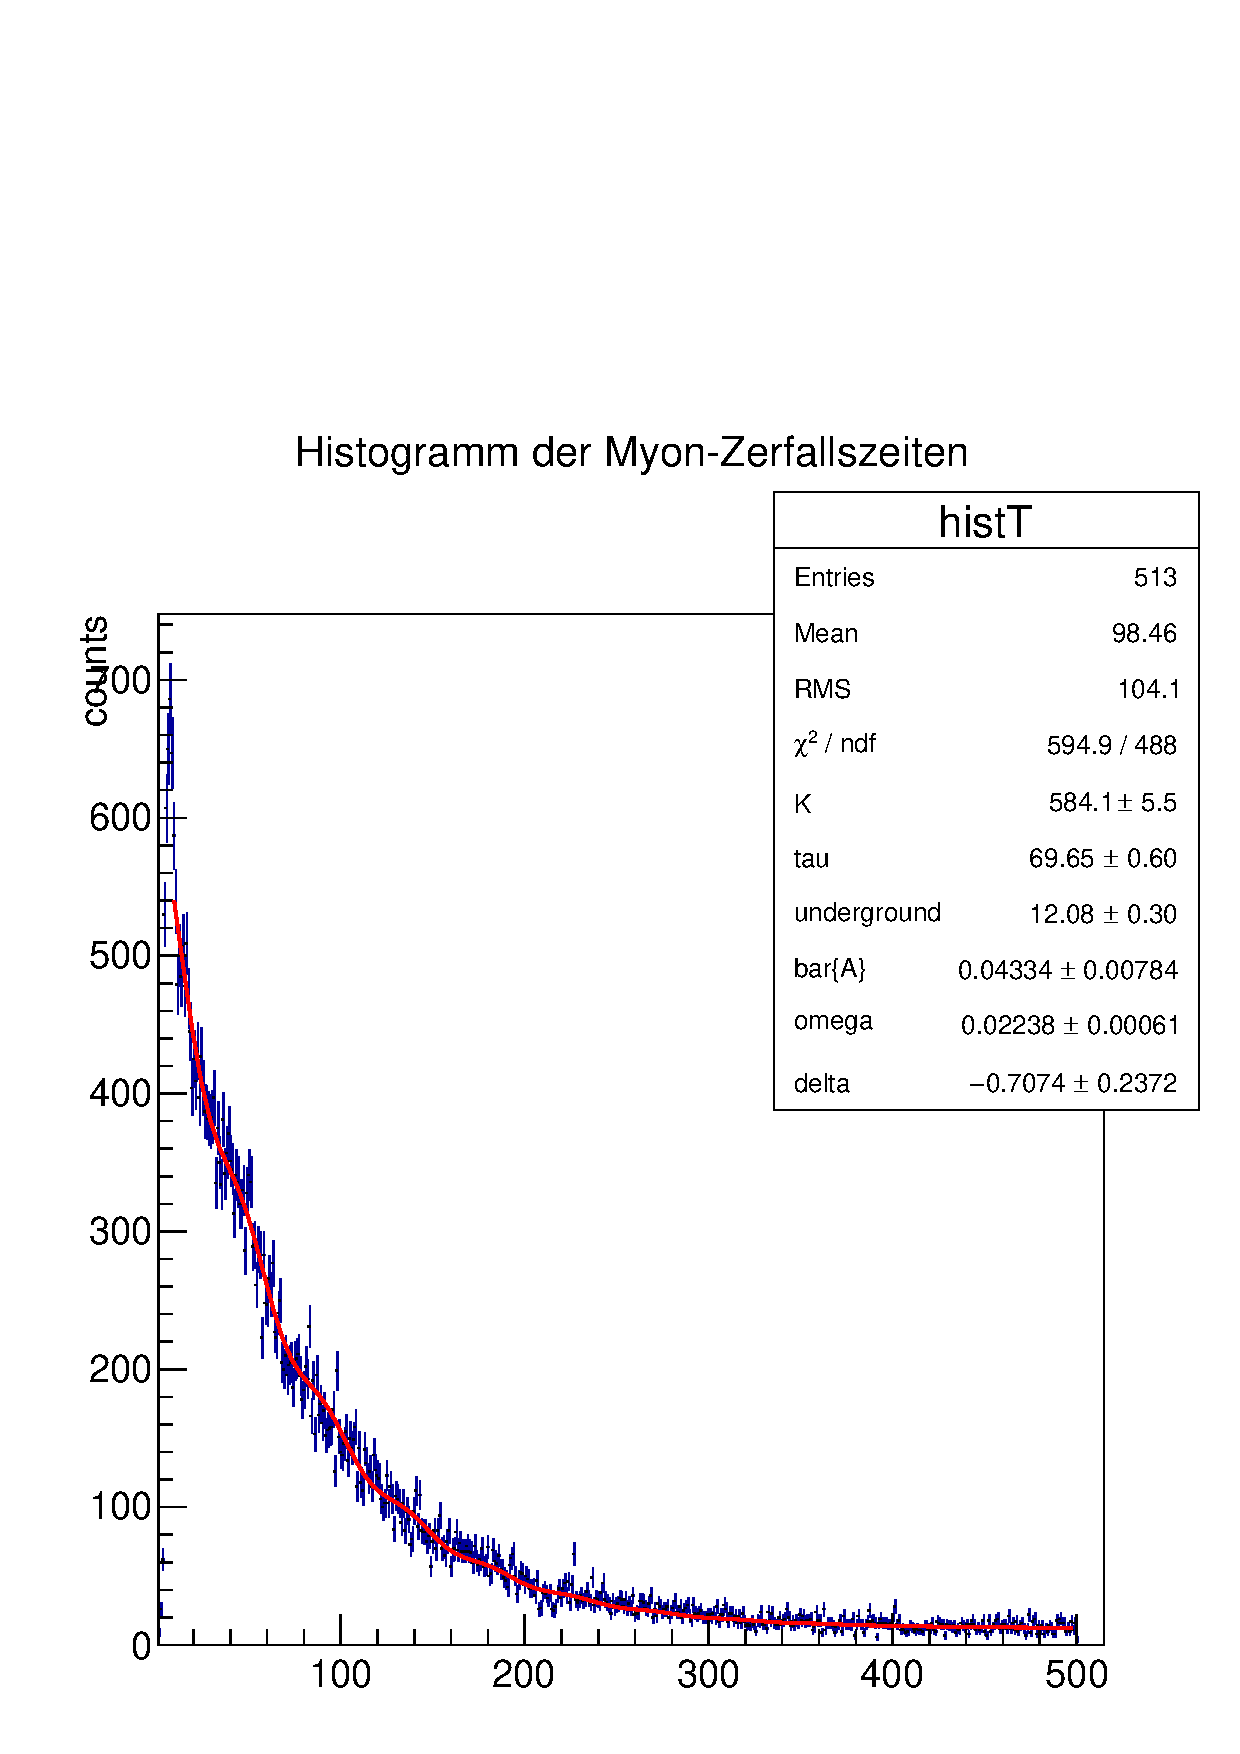
\includegraphics[width=1.1\textwidth]{abbildungen/histogramm.pdf}
  \caption{\textbf{Verteilung der Myon-Zerfallszeiten}
  Eingetragen sind die Zeiten zwischen den Triggersignalen des Szintillators~1 und den
  Signalen aus dem Positron des \APmuon-Zefalls. Die Zeit ist dabei in Kanälen
  aufgetragen und kann nach Gleichung~\ref{eqn:Zeitkalibrierung} in
  Sekunden umgerechnet werden. Zu sehen ist ein exponentieller
  Abfall, wie es bei einem statistischen Prozess zu
  erwarten ist. Zusätzlich kommt es noch zu einer periodischen
  Modulation, da wir nur die Ereignisse selektiert haben, bei denen
  das Positron nach oben emittiert wurde und gleichzeitig ein Magnetfeld angelegt
  hatten. Das Myon emittiert das Positron bevorzugt in Spinrichtung
  und durch die Präzession im Magnetfeld kommt es zur sichtbaren
  Modulation. Damit kann die Präzessionsfrequenz und schließlich der
  Landéfaktor bestimmt werden.}

  \label{fig:zerfallszeiten}
\end{figure}

\clearpage
\subsection{Bedeutung des Landéfaktors}

Der Landéfaktor $g$ gibt für ein Teilchen das Verhältnis des gemessenen magnetischen Moments $ u_{\mathrm{gemessen}}$ zu dem klassisch erwartetem magnetischem Moment $u_{\mathrm{klassisch}}$ an. Demnach gilt

\begin{equation}
g = \frac{ u_{\mathrm{gemessen}} }{u_{\mathrm{klassisch}} } ~.
\end{equation}

Jeder Drehimpuls besitzt in einem Magnetfeld ein magnetisches Moment. Für unterschiedliche Drehimpulse können die Landéfaktoren voneinander abweichen. So ist $g$ für den Bahndrehimpuls eines geladenes Teilchens genau eins, für dessen Spin jedoch $2 + \text{Korrekturen höherer Ordnung}$. Auch negative Werte sind möglich. In einem Magnetfeld mit Betrag $B$ gilt mit der Präzessionsfrequenz $\omega$ und dem Bohrschem Magneton $\mu_\mathrm{B}$

\begin{equation}
g = \frac{\hbar \omega}{\mu_\mathrm{B} B} ~.
\end{equation}

\subsection{Bestimmung des Landéfaktors des Myons}
Aus dem Fit in Abbildung~\ref{fig:zerfallszeiten} der Zerfallszeiten
erhielten wir neben dem Landéfaktor die Präzessionsfrequenz
der Myonen, die mit der Zeitkalibrierung in
Gleichung~\ref{eqn:Zeitkalibrierung}

\begin{equation}
\label{eq:omega}
\omega = \SI{0.671 +-  0.021}{\per\nano\second}
\end{equation}
% (mapcar (lambda (x) (* x  29.9783924)) '(2.23718e-02   6.94896e-4))
% (0.67067059909432 0.0208318649651904)

beträgt. Daraus erhält man den Landéfaktor

% (setq mub 9.27401e-24)
% (setq hbar 1.05457173e-34)
% (setf B 36e-4)
% (/ (* 2 mub B) (* hbar 29.978e9))
% (/ (* hbar 29.978e9 2.24718e-2) (* mub B))2.1278772951876963


\begin{equation}
g = \frac{\hbar \omega}{\mu_B B} = \SI{2.128}{}~.
\end{equation}

Es fehlt noch die Fehlerabschätzung. Da sich der Fehler auf die
Präzessionsfrequenz und auf das Magnetfeld nur multiplikativ auf das
Endergebnis auswirken, bleiben die relativen Fehler erhalten. Mit den
Gleichungen \ref{eqn:inhomogen_fehler} und \ref{eq:omega} erhalten wir

\begin{equation}
  \begin{split}
    \sigma_B &= 7\%\\
    \sigma_{\rm VW} &= 3\%\\
    \sigma_{\omega} &= \frac{\SI{0,021}{}}{\SI{0,671}{}} = 3\%~.\\
  \end{split}
\end{equation}

%(* 0.03 2.128) 0.06384
%(* 0.1 2.128) 0.14896001

Damit haben einen absoluten statistischen Fehler aus dem Fit der Präzessionsfrequenz von \SI{0,06}{} und 
von den systematischen Fehler $\sigma_B$ aus dem Magnetfeld und dem Messfehler des Vorwiderstandes 
durch Fehlerfortpflanzung einen absoluten systematischen Fehler von \SI{0,21}{}. 
Wir erhalten also, nach Rundung auf signifikante Stellen

\begin{equation}
    g = \SI{2.1}{} \pm \SI{0.1}{} \pm \SI{0.2}{}~,
\end{equation}

oder wenn man die systematischen und statistischen Fehler als einen Fehler angibt

\begin{equation}
  \label{eq:g}
    g = \SI{2.1+-0.3}{}~.
\end{equation}

\clearpage

\subsection{Diskussion der Ergebnisse}
Unser Ergebnis für die Lebensdauer von Myonen von 
$\tau_{\rm eff} = \SI{2.08 +- 0.02}{\micro\second}$\eqref{eq:tau}
ist zufriedenstellend. Sie ist damit etwas also niedriger als der in der
Literatur angegebene Wert für die Lebensdauer von freien Myonen, der bei  \SI{2.197}{\micro\second} liegt [\ref{ref:pdg14}], was zum Teil daran liegen könnte, dass wir die effektive Lebensdauer in beinem Material gemessen haben, wo es es im Anfangsbereich bei unter \SI{1}{\micro\second} eine Faltung mit den Elektronen aus dem Zerfall negativer Myonen geben könnte, die eine deutlich geringere Lebensdauer haben. 
Jedoch liegt die Differenz innerhalb der Fehlergrenzen, weshalb das durchaus auch einfach ein durch statistische Unsicherheiten
und systematische Fehler bedingter Effekt sein könte.


Der gemessene Landéfaktor von $g = \SI{2.1+-0.3}{}$
ist ebenfalls sehr gut mit dem theoretisch erwarteten Literaturwert von 2
[\ref{ref:pdg14}] vereinbar. Er ist etwas höher, jedoch liegt die
Abweichung innerhalb der statistischen und systematischen Fehlergrenzen.



\section{Quellen}
\begin{enumerate}
\item Vorbereitungsmappe 
\item \emph{Einführung in das Kernphysikalische Praktikum} von F. K. Schmidt, 
  Überarbeitung von J. Wolf, Ausgabe September 2009. \label{ref:bb}
\item K.A. Olive et al. (Particle Data Group), Chin. Phys. C, 38, 090001 (2014). \label{ref:pdg14}
\end{enumerate}



\end{document}
